API Strategies is based on creation of multiple subtypes of the service.
It uses Strategy design pattern to create a set of implementations that implement the same service definition\@.

The Figure~\ref{fig:strat_structure_and_behaviour} shows the example of the API Strategies.
The service \textit{IgmpPacketWriter} is decomposed into 3 subtypes: \textit{IgmpLeaveGroupWriter},
\textit{IgmpQueryMembershipWriter}, and \textit{IgmpReportMembershipWriter} - each of them implements
the \textit{writePacket} method in a different way.
The subtypes of \textit{IgmpPacketWriter} are also bound to corresponding subtypes of the \textit{IgmpPacket} class
using template parameter \textit{T} that must extend \textit{IgmpPacket} type.
Afterward, specific implementations of the service can work directly with the correct subtype of the packet.
Parts of the implementations that are common in all subtypes of service can be moved to additional abstract
class that realizes \textit{IgmpPacketWriter} interface (using Template design pattern).

\begin{figure}[!htb]
    \centering
    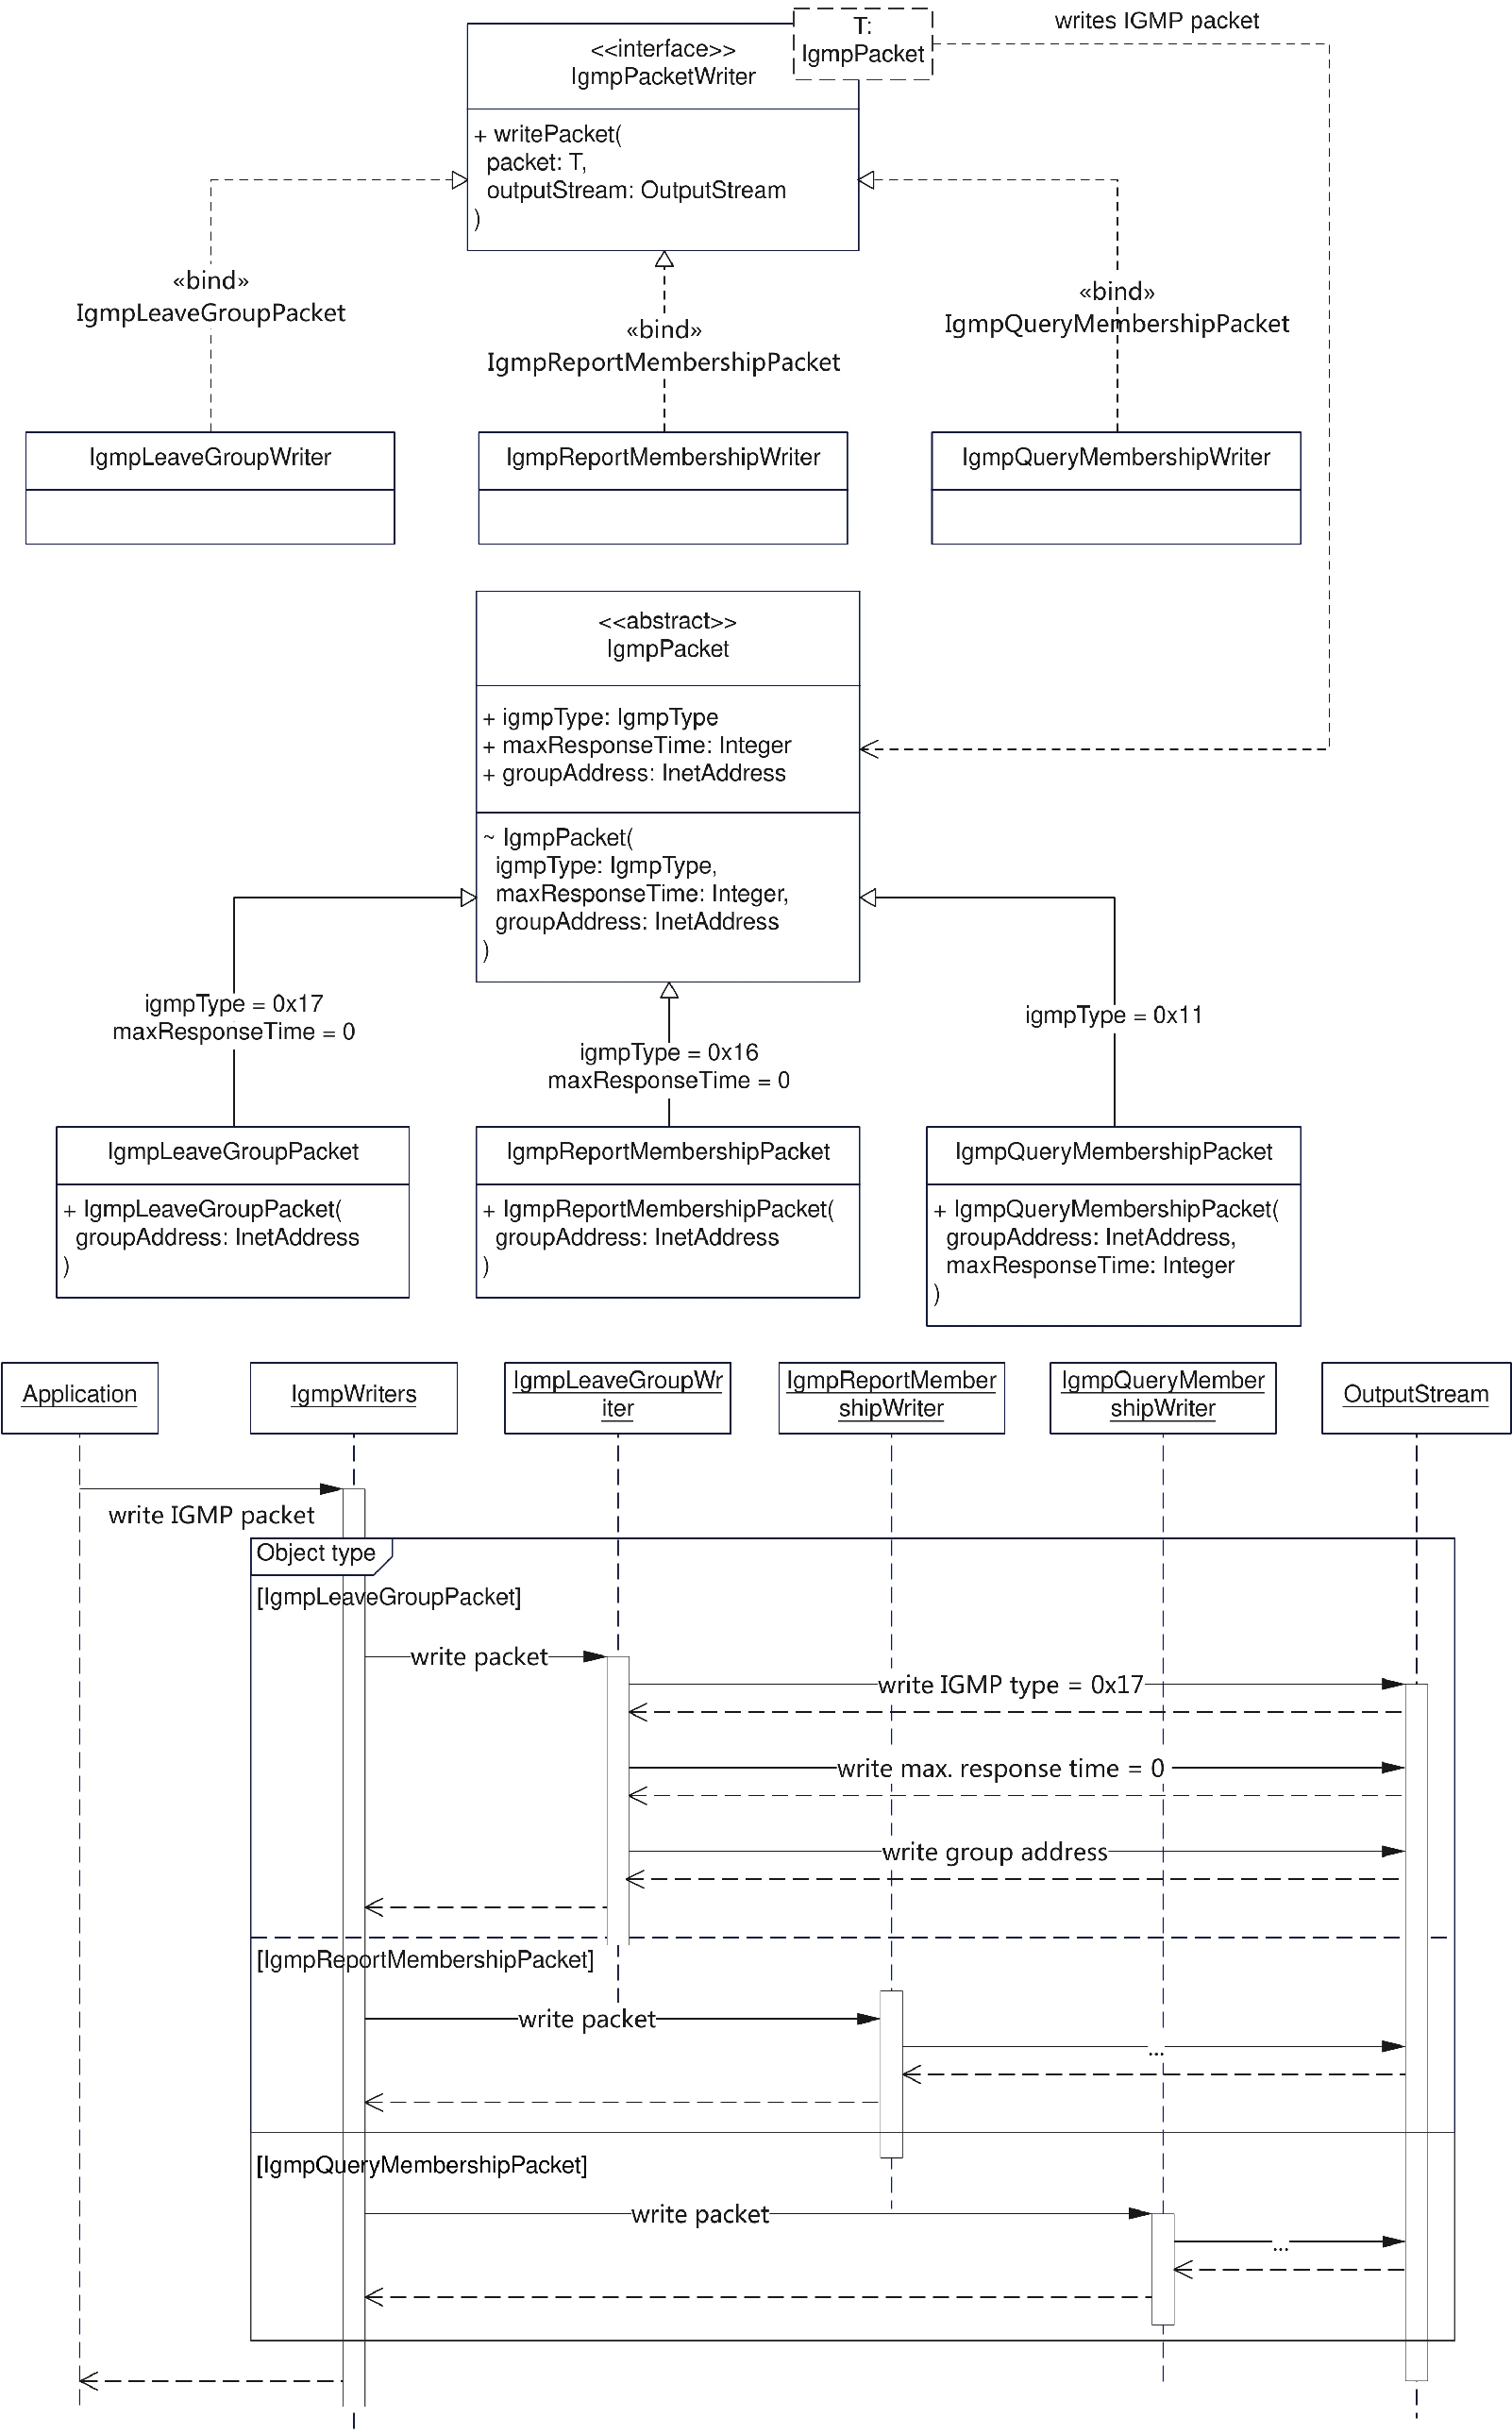
\includegraphics[width=0.85
    \textwidth]{strat_structure_and_behaviour}
    \caption{API Strategies: Decomposition of API into multiple subtypes}
    \label{fig:strat_structure_and_behaviour}
\end{figure}

Benefits of the API Strategies:

\begin{itemize}
    \item This approach can easily be combined with other methodologies that focus on design of interface
    method parameters.
    \item Extensibility of the API - It is possible to add new implementations of the service
    without altering existing implementations.
    \item Testing experimental implementations is much easier using this approach than by passing additional arguments
    to the interface methods or adding new interface methods.
\end{itemize}

Drawbacks of the API Strategies:

\begin{itemize}
    \item Service implementation usually contain also code related to the lifecycle of the service
    (e.g.\ initialization and destruction of the service).
    This lifecycle must be managed for all versions of the service.
    \item Multiple implementations of the service must be distinguished using another identifier.
    This problem is solved by Dependency Injection (DI) framework that supports assigning of the additional qualifier
    to the service implementation.
    \item Maintaining multiple implementations of the service can be difficult because of the code duplication
    between the implementations.
    Usually some parts of the implementation are common in all implementations and can be moved to the template class.
    However, the goal of the API Strategies is to create services implementations that are as isolated as possible.
    This can result in either code duplication or in the creation of additional abstraction layers that are difficult
    to maintain.
    Figure~\ref{fig:strat_infected_tree} shows an example of the more complex service inheritance tree.
\end{itemize}

\begin{figure}[!htb]
    \centering
    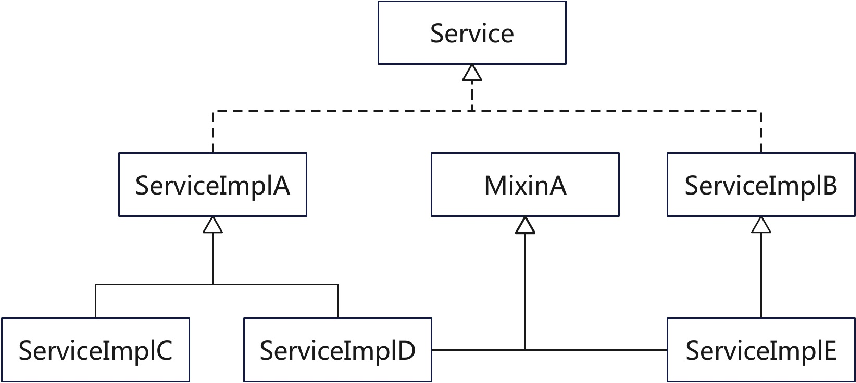
\includegraphics[width=0.66
    \textwidth]{strat_infected_tree}
    \caption{API Strategies: Example of the more complex service inheritance tree}
    \label{fig:strat_infected_tree}
\end{figure}

Common use-cases of the API Strategies:

\begin{itemize}
    \item Multiple implementations in different contexts are required.
    For example, there could be single generic service that defines writing of the packet to the network interface.
    However, there could be multiple types of the network interfaces (e.g.\ Ethernet, Wi-Fi, etc.), each of them
    requiring different strategy for writing the packet to the interface.
    \item There could be multiple implementations of the service that works in different environments.
    For example, the service that performs system calls must be implemented differently under different
    versions of the operating system if certain system calls are different.
    \item Creation of mocked implementations of the service for testing purposes (unit or integration tests).
\end{itemize}
